\documentclass[tikz,border=10pt]{standalone}
\begin{document}
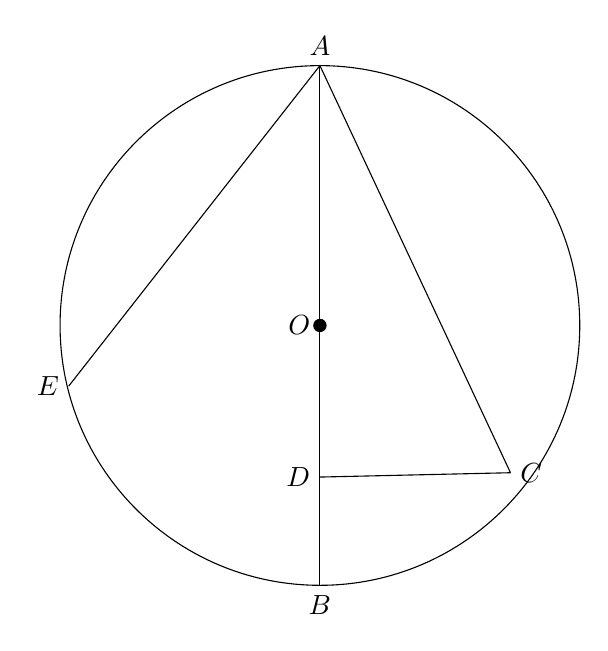
\begin{tikzpicture}[scale=1.1]

\coordinate (O) at (0,0);
\coordinate (A) at (0,3);
\coordinate (B) at (0,-3);
\coordinate (E) at (-2.9,-0.7);
\coordinate (C) at (2.2,-1.7);
\coordinate (D) at (0,-1.75);

\draw (O) circle[radius=3];
\draw (A) -- (B);
\draw (A) -- (E);
\draw (A) -- (C);
\draw (D) -- (C);

\fill (O) circle[radius=2.2pt];

\node[above] at (A) {$A$};
\node[below] at (B) {$B$};
\node[left] at (E) {$E$};
\node[right] at (C) {$C$};
\node[left] at (D) {$D$};
\node[left] at (O) {$O$};

\end{tikzpicture}
\end{document}
